111. \begin{figure}[ht!]
\center{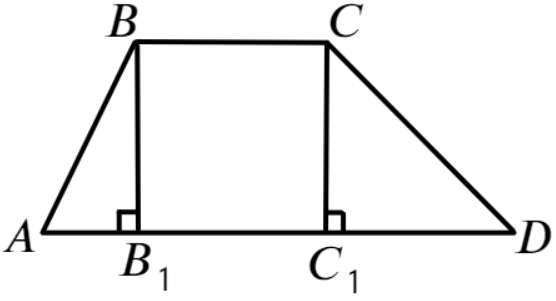
\includegraphics[scale=0.35]{g9-112.png}}
\end{figure}\\
Опустим высоты $BB_1$ и $CC_1.$ Пусть $AB_1=x,$ тогда $C_1D=10-4-x=6-x$ и $BB_1^2=4^2-x^2=CC_1^2=6^2-(6-x)^2,\ 16-x^2=36-36+12x-x^2,\ x=\cfrac{4}{3}.$ Тогда $BB_1=\sqrt{16-\cfrac{16}{9}}=\cfrac{8\sqrt{2}}{3}.$\\
